\documentclass[12pt,a4paper]{extarticle}
\usepackage{../templates/preamble}

\renewcommand{\typeofnum}{4}
\renewcommand{\papertheme}{Многомерные однонаправленные списки.}

\begin{document}
\input{../templates/titlepage.tex}
\setcounter{page}{2}
\tableofcontents
\newpage

% document %
\section{Исходная формулировка задания}
В конец списка l1 добавить все элементы списка l2 в порядке, обратном тому, в котором они встречаются в
списке l2. Т.е. сгруппировать и развернуть список l2.

\section{Определение неясностей}
Просто развернуть список и удалить повторные вхождения недостаточно, необходимо сгруппировать элементы.

\section{Контрольный пример}

\begin{tabularx}{\textwidth}{|t|t|}
    \hline
    \multicolumn{1}{|h|}{Ввод} & \multicolumn{1}{h|}{Вывод} \\ \hline
    {\ttfamily\footnotesize\lstinputlisting{files/in.txt}}
    & {\ttfamily\footnotesize\lstinputlisting[firstline=31]{files/out.txt}} \\ \hline
    {\ttfamily\footnotesize\lstinputlisting{files/in copy.txt}} & \\ \hline
\end{tabularx}

% \section{Ограничения, обусловленные вычислительным устройством}

\section{Формат файлов}
Входные и выходные файлы для маркерного представления должны иметь следующие форматы:

\begin{xltabular}{\textwidth}{|>{\ttfamily\footnotesize}X|}
    \hline
    \multicolumn{1}{|>{\centering\arraybackslash}X|}{Входные файлы} \\ \hline
    [c...c] \\ \hline

    \multicolumn{1}{|>{\centering\arraybackslash}X|}{Выходные файлы} \\ \hline
    l1:\par
    [с...c\par
    |/]\par
    nullptr\par
    \_\_\_\_\_\_\_\par
    l2:\par
    [с...c\par
    |/]\par
    nullptr\par
    \_\_\_\_\_\_\_\par
    Ответ:\par
    [с...c\par
    |/]\par
    nullptr\par\\ \hline
\end{xltabular}

\section{Реализация ввода/вывода}
\begin{xltabular}{\textwidth}{|h|s|s|}
    \hline
    \multicolumn{1}{|h|}{Библиотека} &
    \multicolumn{1}{s|}{Ввод} &
    \multicolumn{1}{s|}{Вывод}\\ \hline
    iostream & cin > > & cout < < \\ \hline
    fstream & istream & ostream \\ \hline
\end{xltabular}

\section{Внутреннее представление данных}

{\centering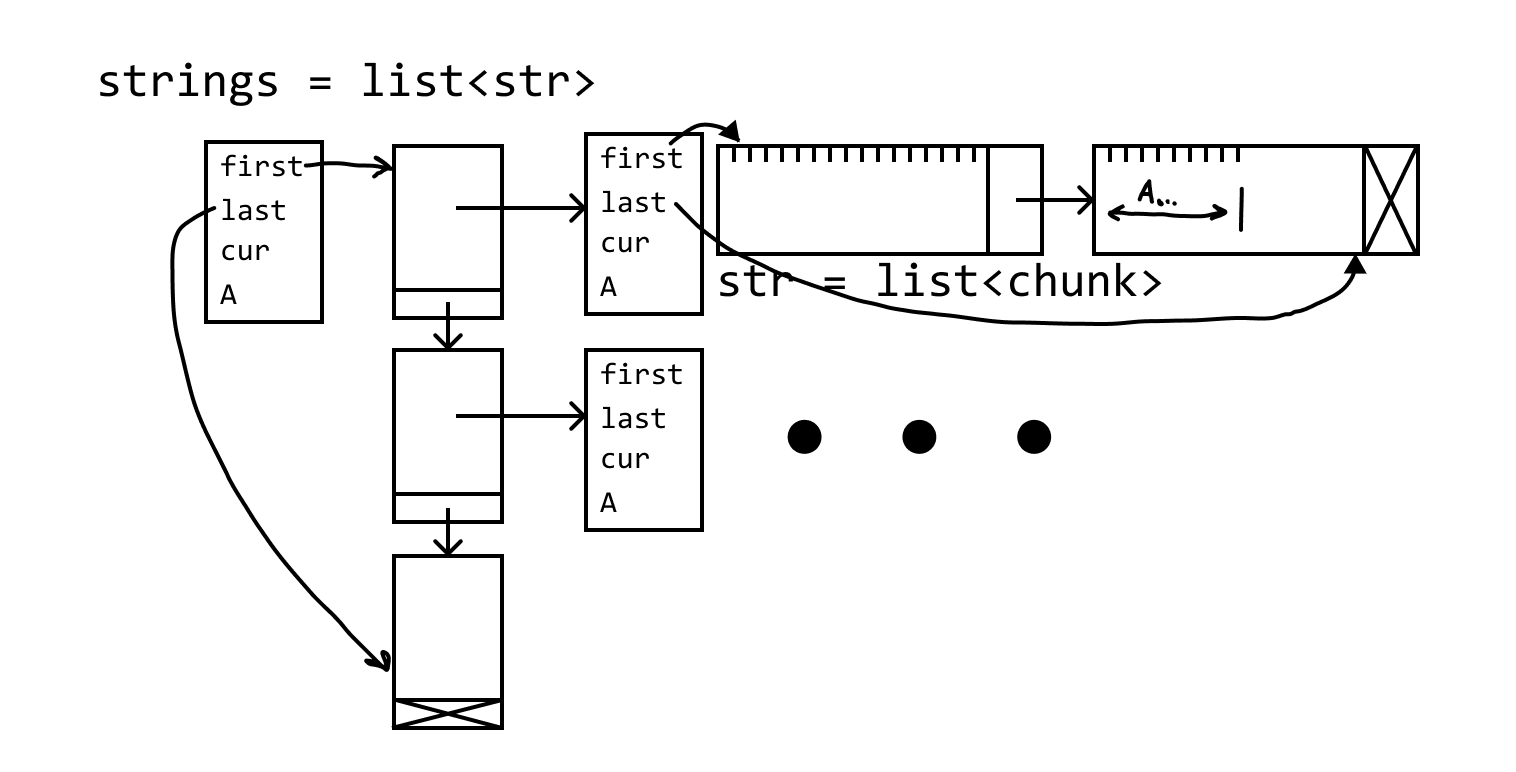
\includegraphics[width=\linewidth]{figures/Frame 19.png}}

\begin{xltabular}{\textwidth}{|
>{\hsize=.2\hsize\centering\arraybackslash\ttfamily\bfseries}X|
>{\hsize=.2\hsize\centering\arraybackslash\itshape}X|
>{\hsize=.6\hsize\centering\arraybackslash}X|
}
\hline
\multicolumn{1}{|>{\hsize=.2\hsize\centering\arraybackslash}X}{Имя переменной} &
\multicolumn{1}{|>{\hsize=.2\hsize\centering\arraybackslash}X}{Тип} &
\multicolumn{1}{|>{\hsize=.6\hsize\centering\arraybackslash}X|}{Описание} \\ \hline
in1, in2 & ifstream & Входные файлы списков \\ \hline
out & ofstream & Выходной файл \\ \hline
l1, l2 & strings & Списки \\ \hline
\end{xltabular}

Структура {\ttfamily\bfseries list} (из {\ttfamily abstracts.hpp}):
\begin{xltabular}{\textwidth}{|
>{\hsize=.2\hsize\centering\arraybackslash\ttfamily\bfseries}X|
>{\hsize=.1\hsize\centering\arraybackslash\itshape}X|
>{\hsize=.7\hsize\centering\arraybackslash}X|}
\hline
\multicolumn{1}{|>{\hsize=.2\hsize\centering\arraybackslash}X}{Имя аргумента} &
\multicolumn{1}{|>{\hsize=.1\hsize\centering\arraybackslash}X}{Тип} &
\multicolumn{1}{|>{\hsize=.7\hsize\centering\arraybackslash}X|}{Описание} \\ \hline
first, cur, last & Node * & Указатели формуляра \\ \hline
Node & struct & Структура нода \\ \hline
A & AT & Дополнительные сведения \\ \hline
\end{xltabular}

Структура {\ttfamily\bfseries list::Node} (из {\ttfamily abstracts.hpp}):
\begin{xltabular}{\textwidth}{|
>{\hsize=.2\hsize\centering\arraybackslash\ttfamily\bfseries}X|
>{\hsize=.1\hsize\centering\arraybackslash\itshape}X|
>{\hsize=.7\hsize\centering\arraybackslash}X|}
\hline
\multicolumn{1}{|>{\hsize=.2\hsize\centering\arraybackslash}X}{Имя аргумента} &
\multicolumn{1}{|>{\hsize=.1\hsize\centering\arraybackslash}X}{Тип} &
\multicolumn{1}{|>{\hsize=.7\hsize\centering\arraybackslash}X|}{Описание} \\ \hline
value & ValueT & Информация \\ \hline
next & Node * & Следующий нод \\ \hline
\end{xltabular}

Структура {\ttfamily\bfseries chunk} (из {\ttfamily types.hpp}):
\begin{xltabular}{\textwidth}{|
    >{\hsize=.2\hsize\centering\arraybackslash\ttfamily\bfseries}X|
    >{\hsize=.3\hsize\centering\arraybackslash\itshape}X|
    >{\hsize=.5\hsize\centering\arraybackslash}X|}
    \hline
    \multicolumn{1}{|>{\hsize=.2\hsize\centering\arraybackslash}X}{Имя аргумента} &
    \multicolumn{1}{|>{\hsize=.3\hsize\centering\arraybackslash}X}{Тип} &
    \multicolumn{1}{|>{\hsize=.5\hsize\centering\arraybackslash}X|}{Описание} \\ \hline
    s & char[CHUNK\_WIDTH] & Кусок строки заданного размера \\ \hline
\end{xltabular}

Шаблон {\ttfamily\bfseries str = list<chunk, \_bar>} (из {\ttfamily types.hpp}):
\begin{xltabular}{\textwidth}{|
>{\hsize=.2\hsize\centering\arraybackslash\ttfamily\bfseries}X|
>{\hsize=.1\hsize\centering\arraybackslash\itshape}X|
>{\hsize=.7\hsize\centering\arraybackslash}X|}
\hline
\multicolumn{1}{|>{\hsize=.2\hsize\centering\arraybackslash}X}{Имя аргумента} &
\multicolumn{1}{|>{\hsize=.1\hsize\centering\arraybackslash}X}{Тип} &
\multicolumn{1}{|>{\hsize=.7\hsize\centering\arraybackslash}X|}{Описание} \\ \hline
arrow & char[4] & Стрелка перехода к очередному элементу \\ \hline
last & int & Длинна последнего нода \\ \hline
\end{xltabular}
Шаблон {\ttfamily\bfseries strings = list<str, \_foo>} (из {\ttfamily types.hpp}):
\begin{xltabular}{\textwidth}{|
>{\hsize=.2\hsize\centering\arraybackslash\ttfamily\bfseries}X|
>{\hsize=.1\hsize\centering\arraybackslash\itshape}X|
>{\hsize=.7\hsize\centering\arraybackslash}X|}
\hline
\multicolumn{1}{|>{\hsize=.2\hsize\centering\arraybackslash}X}{Имя аргумента} &
\multicolumn{1}{|>{\hsize=.1\hsize\centering\arraybackslash}X}{Тип} &
\multicolumn{1}{|>{\hsize=.7\hsize\centering\arraybackslash}X|}{Описание} \\ \hline
arrow & char[5] & Стрелка перехода к очередному элементу \\ \hline
\end{xltabular}

\section{Описание функций}
\subsection{abstracts.ipp}
\subsubsection{Параметры}
\begin{xltabular}
    {\textwidth}{|X|X|X|X|X|X|}
    \hline
    \multirow{2}{0.14\textwidth}{\centering Имя функции} &
    \multicolumn{4}{c|}{Параметры} &
    \multirow{2}{0.14\textwidth}{\centering Возращаемый тип} \\ \cline{2-5}
    & Входные & Выходные & Модифицир. & Транзитные & \\ \hline
    list::Node::Node & & & & & \\ \hline
    list::Node::Node & ValueT val & & & & \\ \hline
    list::Node::operator>>= & const Node\& other & & & & Node * \\ \hline
    list::list & & & & & \\ \hline
    list::is\_empty & & & & & bool \\ \hline
    list::operator== & const list\& other & & & & bool \\ \hline
    list::operator!= & const list\& other & & & & bool \\ \hline
    list::push\_back & Node * node & & node & & void \\ \hline
    list::push\_back & const ValueT\& value & & & value & void \\ \hline
    list::print & ostream\& out & & & & void \\ \hline
    list::destroy & & & & & void \\ \hline
\end{xltabular}

\subsubsection{Функции}
\begin{listed}
    \item list::Node::Node Инициализирует пустой нод или нод со значением
    \item list::Node::operator>>= Возвращает ссылку на нод с таким же значением, как у правого нода, после левого
    \item list::list Инициализирует список
    \item list::is\_empty Проверяет, пустой ли список
    \item list::operator== Оператор сравнения двух списков
    \item list::operator!= Оператор сравнения двух списков
    \item list::push\_back Добавляет нод или новый нод со значением в конец списка
    \item list::print Выводит список в консоль
    \item list::destroy Освобождает память списка
\end{listed}

\subsection{types.сpp}
\subsubsection{Параметры}
\begin{xltabular}
    {\textwidth}{|X|X|X|X|X|X|}
    \hline
    \multirow{2}{0.14\textwidth}{\centering Имя функции} &
    \multicolumn{4}{c|}{Параметры} &
    \multirow{2}{0.14\textwidth}{\centering Возращаемый тип} \\ \cline{2-5}
    & Входные & Выходные & Модифицир. & Транзитные & \\ \hline
    chunk::print & ostream\& out & & out & out & void \& \\ \hline
    chunk::print & ostream\& out, int len & & out & & void \& \\ \hline
    chunk::
    operator== & const chunk\& other & & & & bool \& \\ \hline
    chunk::operator!= & const chunk\& other & & & & bool \& \\ \hline
\end{xltabular}

\subsubsection{Функции}
\begin{listed}
    \item chunk::print Выводит кусок строки в поток.
    \item chunk::operator== Оператор равенства двух чанков
    \item chunk::operator!= Оператор неравенства двух чанков
\end{listed}

\subsection{file.сpp}
\subsubsection{Параметры}
\begin{xltabular}
    {\textwidth}{|X|X|X|X|X|X|}
    \hline
    \multirow{2}{0.14\textwidth}{\centering Имя функции} &
    \multicolumn{4}{c|}{Параметры} &
    \multirow{2}{0.14\textwidth}{\centering Возращаемый тип} \\ \cline{2-5}
    & Входные & Выходные & Модифицир. & Транзитные & \\ \hline
    readline & istream\& in & & in & & str \\ \hline
    readfile & istream\& in & & in & in & strings \\ \hline
    bar & ostream\& out & & out& & void \\ \hline
    process & strings* l1, l2 & & l1, l2 & & void \\ \hline
\end{xltabular}


\subsubsection{Функции}
\begin{listed}
    \item readline Считывание строки с файла
    \item readfile Считывание файла 
    \item bar Вывод линии в поток
    \item process Обработка списков
\end{listed}

\section{Описание алгоритма}
Алгоритм проходится по всем нодам второго списка (с запоминанием следующего) и если нода с таким же значением не было
после первого нода формирующегося списка, то он становится новым первым нодом формирующегося списка, иначе ставится после
нода с таким же значением.

{\centering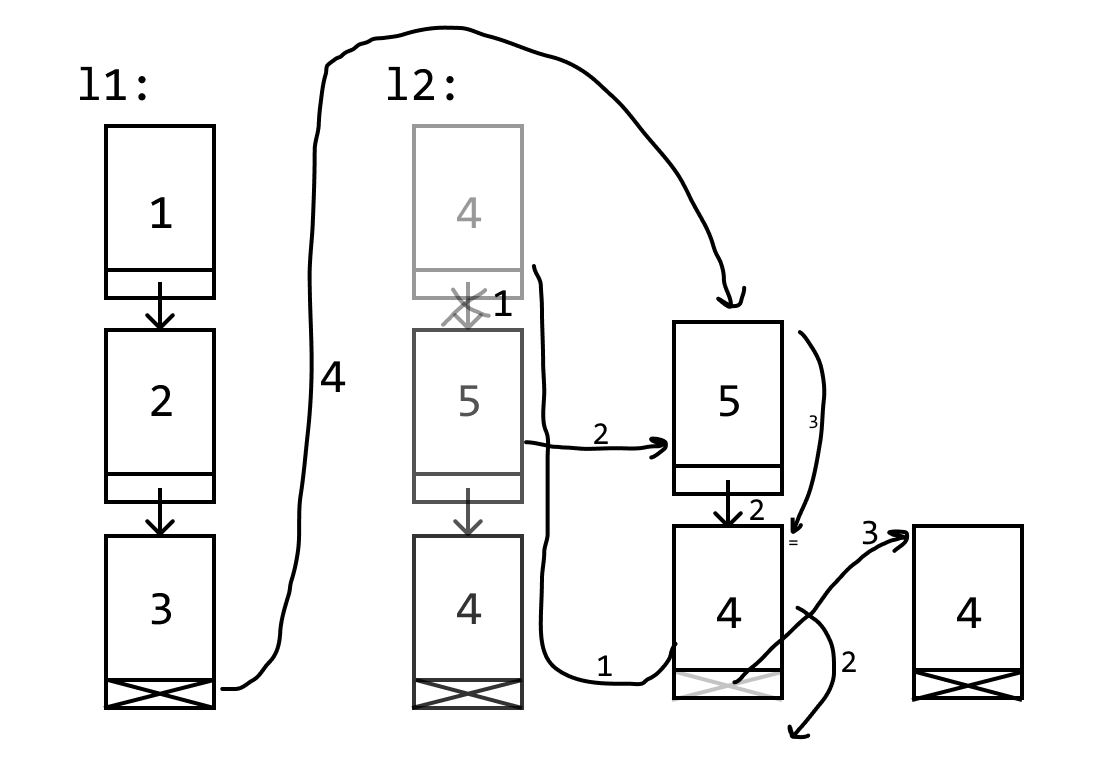
\includegraphics[width=\linewidth]{figures/Frame 20.png}}

Ниже представлены блок-схемы интересных функций.

% 
\includegraphics[width=0.33\linewidth]{figures/main.png}

\includegraphics[width=0.45\linewidth]{figures/process.png}
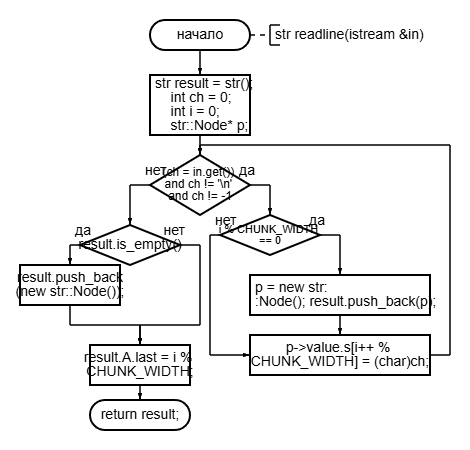
\includegraphics[width=0.5\linewidth]{figures/readline.png}

\section{Исходный код программы}

\begin{xltabular}
    {\textwidth}{X|X}
    abstracts.hpp: \lstinputlisting[language=C++]{../../tasks/4/abstracts.hpp} &
    abstracts.ipp[...-40]: \lstinputlisting[language=C++, lastline=40]{../../tasks/4/abstracts.ipp} \\
\end{xltabular}
\begin{xltabular}
    {\textwidth}{X|X}
    abstracts.ipp[41-68]: \lstinputlisting[language=C++, firstline=41, lastline=68]{../../tasks/4/abstracts.ipp} &
    abstracts.ipp[69-...]: \lstinputlisting[language=C++, firstline=69]{../../tasks/4/abstracts.ipp}\\
\end{xltabular}
\begin{xltabular}
    {\textwidth}{X|X}
    types.hpp: \lstinputlisting[language=C++]{../../tasks/4/types.hpp} &
    types.cpp: \lstinputlisting[language=C++]{../../tasks/4/types.cpp} \\
\end{xltabular}
\begin{xltabular}
    {\textwidth}{X|X}
    file.hpp: \lstinputlisting[language=C++]{../../tasks/4/file.hpp}
    
\includegraphics[width=0.5\textwidth]{figures/chart.png} & 
    file.cpp: \lstinputlisting[language=C++]{../../tasks/4/file.cpp} \\
\end{xltabular}

\begin{center}
\end{center}

\section{Результаты работы программы}
\begin{tabularx}{\textwidth}{|>{\ttfamily\footnotesize}X|>{\ttfamily\footnotesize}X|}
    \hline
    \multicolumn{2}{|X|}{Ввод} \\ \hline
    \multicolumn{2}{|X|}{\lstinputlisting{files/in.txt}\par\lstinputlisting{files/in copy.txt}} \\ \hline
    \multicolumn{2}{|X|}{Вывод} \\ \hline
    \multicolumn{2}{|X|}{\lstinputlisting{files/out.txt}} \\ \hline
\end{tabularx}

\section{Вывод о проделанной работе}
В ходе выполнения работы я научился работе с многомерными однонаправленными списками, разнообразному
перемещению элементов, группировке и сортировке элементов однонаправленного списка.

\end{document}
